\section{Formulation}

An incident electric field $\vb{E}_\text{inc}(\vb{r}, t)$ induces a source polarization distribution, $\vb{P}(\vb{r}, t)$, on a collection of objects (either discrete or continuous) embedded in a homogeneous background medium by way of an underlying linear~\cite{} or nonlinear~\cite{Glosser2017} process.
This current subsequently generates a secondary $\vb{E}_\text{scat}(\vb{r}, t) = \mathfrak{F}\qty{\vb{P}(\vb{r}, t)}$, thus the total field at any spacetime coordinate becomes
\begin{equation}
  \vb{E}(\vb{r}, t) = \vb{E}_\text{inc}(\vb{r}, t) + \mathfrak{F}\qty{\vb{P}(\vb{r}, t)}.
\end{equation}
Assuming $\vb{E}(\vb{r}, t)$ consists of a low-frequency envelope modulated by a high-frequency sinusoid, i.e. $\vb{E}(\vb{r}, t) = \tilde{\vb{E}}(\vb{r}, t) e^{i \omega_L t}$, we can suppress the $e^{i \omega_L t}$ term in favor of an assumed spatial phase factor.
Thus,
\begin{equation}
  \tilde{\vb{E}}(\vb{r}, t) = \tilde{\vb{E}}_\text{inc}(\vb{r}, t) + \tilde{\mathfrak{F}}\qty{\tilde{\vb{P}}(\vb{r}, t)}
\end{equation}
where tildes on field variables denote envelope functions.
By enforcing radiation boundary conditions (namely that $\vb{E}_\text{scat}(\vb{r}, t) \to 0$ as $\abs{\vb{r}} \to \infty$), Maxwell's equations require
\begin{equation}
  \mathfrak{F}\qty{\vb{P}(\vb{r}, t)} = -\frac{\mu}{4\pi} \siint \frac{\delta(t_R - t')}{\abs{\vb{r} - \vb{r}'}} \qty(\pdv[2]{{t'}} - c^2 \grad' \grad'\boldsymbol{\cdot}) \vb{P}(\vb{r}', t') \dd[1]{t'} \dd[3]{\vb{r}'}
  \label{eq:efie}
\end{equation}
where $\mu$ characterizes the permeability of the background medium and $t_R \equiv t - \abs{\vb{r} - \vb{r}'}/c$ (see \cref{appendix:vector wave equation}).
Accordingly,
\begin{equation}
  \tilde{\mathfrak{F}}\qty{\tilde{\vb{P}}(\vb{r}, t)}e^{i \omega_L t} = -\frac{\mu}{4\pi} \siint \frac{\delta(t_R - t')}{\abs{\vb{r} - \vb{r}'}} \qty(\pdv[2]{{t'}} - c^2 \grad' \grad'\boldsymbol{\cdot}) \tilde{\vb{P}}(\vb{r}', t') e^{i \omega_L t'} \dd[1]{t'} \dd[3]{\vb{r}'}
  \label{eq:efie envelope}
\end{equation}
and, after performing the temporal integration and suppressing the $e^{i \omega_L t}$ factor on both sides of the equation, we have
\begin{equation}
  \tilde{\mathfrak{F}}\qty{\tilde{\vb{P}}(\vb{r}, t)} = -\frac{\mu}{4\pi} \sint \frac{e^{- i \omega_L \abs{\vb{r} - \vb{r}'}}}{\abs{\vb{r} - \vb{r}'}} \qty(\pdv[2]{t} + 2 i \omega_L \pdv{t} - \omega_L^2 - c^2 \grad' \grad'\boldsymbol{\cdot}) \tilde{\vb{P}}(\vb{r}', t_R) \dd[3]{\vb{r}'}.
  \label{eq:efie envelope}
\end{equation}
(We note that $\partial_{t_R} = \partial_{t}$ and that \cref{eq:efie envelope} recovers \cref{eq:efie} in the limit of $\omega_L \to 0$.)

To effect the calculation of \cref{eq:efie envelope} on bounded geometries of interest, we represent $\tilde{\vb{P}}(\vb{r}, t)$ as a collection of spatio-temporal basis functions,
\begin{equation}
  \tilde{\vb{P}}(\vb{r}, t) \approx \sum_{\ell = 0}^{N_s - 1} \sum_{m = 0}^{N_t - 1} \tilde{\mathcal{A}}_\ell^{(m)} \vb{s}_\ell(\vb{r}) T(t - m \, \Delta t).
  \label{eq:discretization}
\end{equation}
Conventionally, $\Delta t^{-1} \propto \omega_\text{max}$---the highest frequency in the system.
By formulating the problem in terms of envelope functions, however, we may choose $\Delta t$ proportional to the bandwidth of the envelopes.
In narrowband applications that evade a frequency-domain analysis---such as those with nonlinear (semiclassical) trappings---this can allow a $\Delta t$ several orders of magnitude larger than in conventional simulations.
This envelope shifting approach does not work equally well in space, however; due to the presence of the $e^{i \omega_L \abs{\vb{r} - \vb{r}'}/c}$ factor in \cref{eq:efie envelope}, interference phenomena still occur on the scale of $\omega_L/c$ (i.e. at a high spatial frequency), thus we still require sub-wavelength spatial discretizations.
Finally, we require both $\vb{s}_\ell(\vb{r})$ and $T(t)$ to have finite support, and $T(t)$ must accurately interpolate derivatives of order $0 \leqslant d \leqslant 2$ to capture the full dynamics of \cref{eq:efie envelope}.

Substituting \cref{eq:discretization} into \cref{eq:efie envelope} and projecting onto the same set of $\vb{s}_\ell(\vb{r})$ produces a spatially-blocked matrix equation of the form
\begin{equation}
  \begin{aligned}
    \tilde{\mathcal{F}}^{(m)} &= \tilde{\mathcal{L}}^{(m)} + \sum_{m'= 0}^m \tilde{\mathcal{Z}}^{(m - m')} \tilde{\mathcal{A}}^{(m')} \\
  \end{aligned}
  \label{eq:mot}
\end{equation}
where
\begin{subequations}
  \begin{align}
    \tilde{\mathcal{F}}^{(m)}_\ell &= \langle \vb{s}_\ell(\vb{r}), \tilde{\vb{E}}(\vb{r}, m \, \Delta t) \rangle \label{eq:f elements}\\
    \tilde{\mathcal{L}}^{(m)}_\ell &= \langle \vb{s}_\ell(\vb{r}), \tilde{\vb{E}}_\text{inc}(\vb{r}, m \, \Delta t) \rangle \label{eq:l elements}\\
    \tilde{\mathcal{Z}}^{(k)}_{\ell\ell'} &= \langle \vb{s}_\ell(\vb{r}), \tilde{\mathfrak{F}}\qty{\vb{s}_{\ell'}(\vb{r}, T(k \, \Delta t)} \rangle \label{eq:z elements}.
  \end{align}
\end{subequations}

For finite systems, only $\tilde{\mathcal{Z}}^{(0)}$ through $\tilde{\mathcal{Z}}^{(N_d)}$ contain nonzero elements, corresponding to the $N_d$ timesteps required to traverse the system completely.
Immediately, this bands $\tilde{\mathcal{Z}}$ to reduce the complexity of the sum in \cref{eq:mot} though the $\mathcal{O}(N_s^2)$ spatial complexity still dominates the overall computational cost.
Consequently, we draw inspiration from FFT-based techniques such as the Adaptive Integral Method (AIM)~\cite{Bleszynski1996,Yilmaz2004}, Conjugate Gradient FFT (CG-FFT)~\cite{CG-FFT}, and Particle-Particle Particle-Mesh (P$^3$M)~\cite{p cubed m} to develop an accelerated methodology for evaluating \cref{eq:mot}.

\subsection{Auxiliary grids}

\begin{figure}
  \centering
  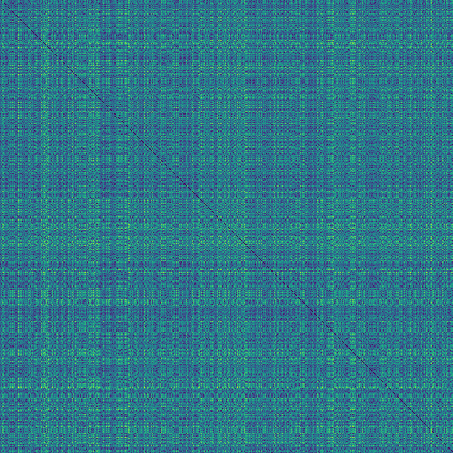
\includegraphics[width=0.4\textwidth]{figures/dist_mat_unsorted}
  \hspace{1cm}
  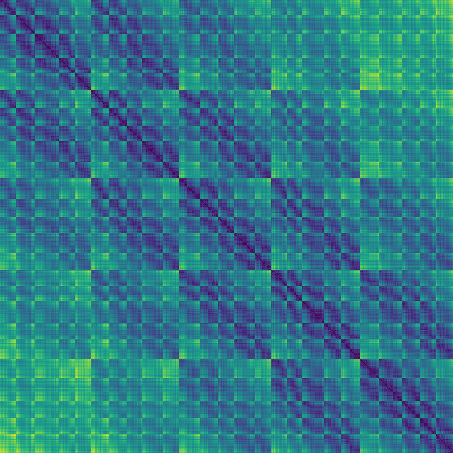
\includegraphics[width=0.4\textwidth]{figures/dist_mat_sorted}
  \caption{\label{fig:matrix structure} The Laplace-kernel interaction matrix between 1024 points in a unit cube appears to have very little structure (left).
    While we cannot fully order the points in three dimensions, we \emph{can} permute the matrix so as to give points within the same neighborhood adjacent indices.
    Points ordered thusly produce a diagonally-dominant interaction matrix with a hierarchical Toeplitz substructure (right).
    Such structures indicate portions of the matrix have very accurate low-rank approximations, offering the possibility of significant compression.
  }
\end{figure}

\begin{figure}
  \centering
  \usetikzlibrary{colorbrewer, decorations.pathreplacing, shapes}

\begin{tikzpicture}[>=latex, scale=2]
\draw[step=1, black, thick, opacity=0.1] (-2,-2) grid (3, 3);

\fill[cbblue, opacity=0.4] (0,0) rectangle (1, 1);
\fill[cbblue, opacity=0.2] (-1,-1) rectangle (2, 2);

\foreach \x in {-1,...,2} {
  \foreach \y in {-1,...,2} {

    \draw[thick, cbblue, fill=white, radius=0.1] (\x,\y) circle;

  }
}


\fill[cbblue, radius=0.03] (0.2, 0.7) node (A) {} circle;
\fill[cbblue, radius=0.03] (0.5, 0.2) node (B) {} circle;
\fill[cbblue, radius=0.03] (0.8, 0.5) node (C) {} circle;

\foreach \x in {0, 0.333, ..., 1} {
  \foreach \y in {0, 0.333, ..., 1} {
    %\draw[cbblue, fill=white] (\x,\y) circle (0.05);
    %\draw[] (\x,\y) node[cross, cbblue] {};
  }
}

\draw[diamond] (1.5, 1.5);

%\draw (0.5, 0.5) node[cross out] {} circle (0.2);

\fill[cbblue, radius=0.06] node[anchor=north east] (0, 0) {$\mathbf{r}_\text{box}$} circle;

\node[cbblue] (pts) at (0.5, 1.2) {Particles};
\draw[cbblue, ->] (pts) -- (A);
\draw[cbblue, ->] (pts) -- (B);
\draw[cbblue, ->] (pts) -- (C);

\draw[cbblue, thick, decorate,decoration={brace,amplitude=10}] (-1.1,2.2) -- (2.1, 2.2) node [midway, above, yshift=10] {Expansion region};
\draw[cbblue, thick, decorate,decoration={brace,amplitude=10}] (1.1,1.1) -- (1.1, -0.1) node [midway, right, xshift=10] {Box};

\draw[<->, cbblue] (-2, -1.8) -- (-1, -1.8) node [midway, fill=white] {$s_x$};
\draw[<->, cbblue] (-1.8, -2) -- (-1.8, -1) node [midway, fill=white] {$s_y$};

\end{tikzpicture}

  \caption{\label{fig:aim terminology} Illustration of an AIM box and the surrounding environment.
    All of the sources within a box (shown as the central shaded square) map to the same set of expansion points (shown as open circles) indexed relative to $\vb{r}_\text{box} = \floor{\vb{r}/s}$.
  }
\end{figure}

\begin{figure}
  \centering
  \conditionalFigureInput{figures/expansion-grid}
  \caption{\label{fig:expansion grid}Spatial expansion pattern for a two-dimensional system.
    An expansion of order $m$ requires $(m + 1)^3$ grid points.
    Moreover, increasing the expansion order incorporates new points in such a way as to keep $\vb{s}_\ell(\vb{r})$ as close to the center of the expansion region as possible.
  }
\end{figure}

\begin{figure}
  \centering
  \conditionalFigureInput{figures/nf_correction}
  \caption{\label{fig:nearfield correction}Expansions $A$ and $B$ overlap, but only box $B$ lies in the nearfield of box $C$.
    Consequently, we must track the $BC$ interaction (dashed line) independently of the FFT-based convolution so as to remove its high-error contribution to the total field.
  }
\end{figure}

To effect a sub-quadratic calculation of \cref{eq:mot}, we approximate $\tilde{\mathcal{Z}}^{(k)}$ as a sum of near- and far-field contributions.
The near-field matrix elements follow directly from \cref{eq:z elements}---sources within a prescribed distance threshold interact ``directly'' so as to avoid incurring large errors in potentials with singularities.
In contrast, the far-field matrix never explicitly arise.
Instead, we construct the far-field interaction matrices between auxiliary sources residing on a regular grid.
Such a procedure has two salient advantages: it compresses the interaction matrix to a reduced number of auxiliary unknowns and imposes a Toeplitz structure amenible to diagonalization with fast Fourier transforms (FFTs).

The original AIM scheme in~\cite{Bleszynski1996} embeds a scattering structure within an auxiliary rectangular grid.
By construction, the interaction matrix of a translationally-invariant propagator (such as \cref{eq:efie envelope}) on this grid will have a hierarchical (block) Toeplitz structure.
This structure affords a very efficient matrix multiplication: as this matrix represents a discrete convolution, a multidimensional FFT diagonalizes the entire matrix in $\mathcal{O}(n \log n)$ steps.

Effecting this calculation for arbitrary structures requires one additional step, however.
As structures do not, in general, reside on structured grids, we require

\begin{enumerate}
  \item \textbf{Projection:} At time $m \, \Delta t$, we project the $\tilde{\mathcal{A}}^{(m)}_\ell \vb{s}_\ell(\vb{r})$ quantities onto a collection of spatial $\delta$-functions (the exterior grid).
    The number expansion points for each $\vb{s}_\ell(\vb{r})$ depends on the number of multipole moments required to recover the potential to a prescribed accuracy at a given distance away from $\vb{s}_\ell(\vb{r})$.
  \item \textbf{Propagation:}
  \item \textbf{Back-projection:}
  \item \textbf{Correction:}
  \item \textbf{Interpolation:}
\end{enumerate}

\section{Moment-matching}

To facillitate FFT-based matrix-vector products, we represent the primary $\vb{s}_\ell(\vb{r})$ basis functions as a weighted sum of $\delta$-functions on the surrounding gridpoints, i.e.
\begin{equation}
  \psi_\ell(\vb{r}) \approx \sum_{\vb{u} \in B_{\ell}} \Lambda_{\ell\vb{u}} \delta(\vb{r} - \vb{u}).
  \label{eq:grid linear combination}
\end{equation}
Here, $\psi_\ell(\vb{r}) \in \qty{\vb{s}_\ell(\vb{r})\cdot \vu{x}, \vb{s}_\ell(\vb{r}) \cdot \vu{y}, \vb{s}_\ell(\vb{r}) \cdot \vu{z}}$ and $B_\ell$ denotes the collection of grid points, $\vb{u}$, within the expansion region of $\vb{s}_\ell(\vb{r})$.
For an expansion of order\footnote{In principle, one could expand to different orders in different cartesian directions, though this involves considerably more bookkeeping for relatively little benefit. Thus, for convenience, we take ``the expansion order'' to mean the expansion order in every direction.} $m$, this sum contains $(m + 1)^3$ terms corresponding to the $(m + 1)^3$ grid points nearest to $\vb{s}_\ell(\vb{r})$.
Consequently, the $\Lambda_{\ell \vb{u}}$ matrices contain few nonzero elements and we have elected to use a moment-matching scheme to capture the $(m + 1)^3$ multipole moments of $\vb{s}_\ell(\vb{r})$ according to
\begin{equation}
  \sint (x - x_0)^{m_x}(y - y_0)^{m_y}(z - z_0)^{m_z} \qty[\psi_\ell(\vb{r}) - \sum_{\vb{u} \in c_\ell}\Lambda_{\ell\vb{u}}\delta(\vb{r} - \vb{u})] \dd[3]{\vb{r}} = 0.
  \label{eq:moment matching}
\end{equation}
In this expression, $0 \leqslant m_x, m_y, m_z \leqslant m$ and $\vb{r}_0 \equiv x_0 \vu{x} + y_0 \vu{y} + z_0\vu{z}$ denotes the origin about which we compute the multipoles.
Thus, to calculate the $\Lambda_{\ell \vb{u}}$, we solve the least-squares system,
\begin{equation}
  \sum_{\vb{u} \in B_\ell} W_{\vb{m}\vb{u}}\Lambda_{\ell\vb{u}} = Q_{\ell\vb{m}},
  \label{eq:expansion matrix system}
\end{equation}
where
\begin{subequations}
  \begin{align}
    W_{\vb{m}\vb{u}} &= (u_x - x_0)^{m_x} (u_y - y_0)^{m_y} (u_z - z_0)^{m_z} \label{eq:w matrix} \\
    Q_{\ell \vb{m}} &= \int_{} \psi_\ell(\vb{r}) (x - x_0)^{m_x} (y - y_0)^{m_y} (z - z_0)^{m_z} \dd[3]{\vb{r}} \label{eq:q vector}.
  \end{align}
\end{subequations}
With infinite precision, the choice of $\vb{r}_0$ merely sets a reference point for the multipole coordinate system; to minimize numerical issues, however, we choose $\vb{r}_0$ at the center of $\vb{s}_\ell(\vb{r})$.
As the primary basis functions consist entirely of $\delta$-functions, $\vb{r}_0 = \vb{r}$ and $Q_{\ell\vb{m}} = 0$ everywhere except for $Q_{\ell \vb{0}} \equiv 1$.


\subsection{Spatial analysis}

Consider two point particles located at $x_\text{src}$ and $x_\text{obs}$.
A time-independent Green's function, $g(x_\text{obs} - x_\text{src})$, describes the interaction between the two particles and we wish to construct a polynomial approximation of $g(x - x_\text{src})$ for $x$ in the vicinity of $x_\text{obs}$ as in \cref{fig:1d moments}.

To construct an interpolation polynomial over the expansion region of order $M$, we define a polynomial coordinate $x_p$ in units of $h$ such that $x_p^\text{min} \leqslant x_p \leqslant x_p^\text{min} + M$ where $x_p^\text{min} \equiv -\floor*{M/2}$.
Consequently, the expansion points about $x_\text{obs}$ correspond to $x_p \in \{-\floor*{M/2}$, $-\floor*{M/2} + 1$, $-\floor*{M/2} + 2$, $\ldots\}$ with the \nth{0} order expansion point, $x_0$, equivalent to $x_p = 0$.
Such a coordinate system defines the Vandermonde linear equation $\sum_{j}V_{ij} w_j = g_i$ for the weights of an interpolating polynomial\footnote{In principle this analysis works equally well in the original $(x_\text{src}, x_\text{obs})$ coordinate system. The polynomial coordinate has three advantages, however: it indexes the expansion points ``logically'' from left to right, $x_p^\text{min} \in \mathbb{Z}$ and thus the Vandermonde matrix has infinite precision, and it makes the interpolation error in terms of $h$ explicit.}~\cite{NumericalRecipes} where
\begin{subequations}
  \begin{align}
    V_{ij} &= (x_p^\text{min} + i)^j \\
    g_i &= g\qty((x_0 - x_\text{src}) + h(x_p^\text{min} + i))
  \end{align}
\end{subequations}
and $0 \leqslant i, j \leqslant M$.
Approximating $g(x - x_\text{src})$ at $x_\text{obs}$ then becomes a matter of evaluating this polynomial at $x_p = \qty(x_\text{obs} - x_0)/h$, i.e.
\begin{equation}
  g(x_\text{obs} - x_\text{src}) \approx \sum_{i = 0}^{M} w_i \qty(\frac{x_\text{obs} - x_0}{h})^i.
\end{equation}
Accordingly, the polynomial approximation to $g(x_\text{obs} - x_\text{src})$ contains terms of order $\mathcal{O}(h^{-M})$ and we can expect the approximation error to scale as $\mathcal{O}(h^{-(M + 1)})$ as demonstrated in \cref{fig:grid convergence}.
This also motivates using the approximation to calculate interactions involving differential operators; applying an $n^\text{th}$-order derivative reduces the polynomial order by $n$, thus the error scales like $\mathcal{O}(h^{-(M + 1) + n})$.

\begin{figure}
  \centering
  \usetikzlibrary{decorations.markings}
\tikzset{
    mark position/.style args={#1(#2)}{
        postaction={
            decorate,
            decoration={
                markings,
                mark=at position #1 with \coordinate (#2);
            }
        }
    }
}

\begin{tikzpicture}[scale=1.7]

\foreach \i in {0, ..., 4}
{
  \draw[thick] (\i, -0.6) -- (\i, 0.6);
}

\fill[green!60!black] (0,0) circle (0.1) node [anchor=north west] {$x_\text{src}$};
\fill[green!40!black] (7.2,0) circle (0.1) node [anchor=north west] {$x_\text{obs}$};

\draw[thick, blue] (7,-0.6) node[below]{$x_0$} -- (7, 0.6) node[above]{$m = 0$};
\draw[thick, blue!75!red] (8,-0.6) node[below]{$x_1$} -- (8, 0.6) node[above]{$m = 1$};
\draw[thick, blue!50!red] (6,-0.6) node[below]{$x_2$} -- (6, 0.6) node[above]{$m = 2$};
\draw[thick, blue!25!red] (9,-0.6) node[below]{$x_3$} -- (9, 0.6) node[above]{$m = 3$};
\draw[thick, blue!0!red] (5,-0.6) node[below]{$x_4$} -- (5, 0.6) node[above]{$m = 4$};

\draw[dashed, thick, orange, mark position=0.9(g)] plot [smooth] coordinates {(4.8, -0.5) (5,-0.4) (6, 0.3) (7, 0.1) (8, 0.4) (9, -0.3) (9.2, -0.4)};
%\node[orange, anchor=west] (g) at (9.2, -0.4) {$g(x-x_\text{src})$};

\end{tikzpicture}

  \caption{\label{fig:1d moments} Polynomial interpolation of $g(x - x_\text{src})$ near $x_\text{obs}$.
    Here, the green curve represents the actual $g(x - x_\text{src})$ and the dashed black line its approximation.
    Evaluating the $n^\text{th}$-order approximation requires knowledge of the signal at $n + 1$ grid points surrounding $x_\text{obs}$.
  }
\end{figure}

\begin{figure}
  \centering
  \begin{filecontents}{grid_spacing.dat}
Spacing             	Order0            	Order1              	Order2                	Order3                	Order4                 
0.2                 	10.311922586843853	6.547888556532848   	0.8078593676582986    	0.6900135622760024    	0.07775624373511587    
0.1861144081859398  	13.420661187167552	2.114064129983551   	0.5176983592090901    	0.3090021241170343    	0.047645445263203585   
0.17319286467201306 	16.28770034601291 	2.035108560409383   	0.4080937775243047    	0.24403206604795324   	0.10482680642842229    
0.16116843755229637 	8.519866354241426 	4.322198387023356   	0.3818170863654957    	0.2885417655222987    	0.02599109071836223    
0.14997884186649116 	8.216773910589568 	1.5357193391783812  	0.9111449652707617    	0.0870040561818314    	0.03892261096436527    
0.13956611697197327 	7.91364029423806  	1.3559066034348457  	0.2965904337336443    	0.1338093251221245    	0.03031081459048604    
0.12987632631524226 	7.475948204162177 	3.1937563384698953  	0.159787816142875     	0.1277975497486948    	0.007284023505291419   
0.12085927804762657 	6.5376413460444045	1.0567180589163159  	0.1365885118608641    	0.07980974374631232   	0.005047801515746074   
0.11246826503806982 	8.194864043013252 	2.264107617481496   	0.6967763929264409    	0.06850903937472122   	0.003057730482123484   
0.10465982293629894 	8.090874834317837 	0.609830973952806   	0.1880026044216161    	0.024048270774990978  	0.007851108795157513   
0.09739350503317262 	11.567176061843169	0.31523828541460563 	0.28331122679347015   	0.012044396686557947  	0.003518944334057881   
0.09063167275201636 	5.0412382168658825	1.0800851897321575  	0.16008918930196203   	0.01288087194156884   	0.0019306677426391755  
0.08433930068571645 	5.878811112707047 	0.5350738193040928  	0.19041019791876324   	0.005194902372171951  	0.002032009900824846   
0.07848379516969071 	4.189910886513379 	0.5756267428004771  	0.11451555388096576   	0.008271411808739722  	0.0012716498146993934  
0.07303482545096754 	4.871506522285374 	0.22727569303236173 	0.02228380547005147   	0.013159246477990934  	0.00029382849770544987 
0.06796416657885118 	4.810718548949396 	0.8587931609444456  	0.04436555600335379   	0.009426219732028694  	0.0004953588769775904  
0.06324555320336758 	5.118235369183121 	0.1330037964356479  	0.01481795934173761   	0.007348233701952196  	0.0001619123841881273  
0.058854543524185635	3.3092417760722395	0.6500461502198256  	0.08053291827668115   	0.005614857608020859  	0.00034058332297163483 
0.05476839268528723 	5.461374355999743 	0.09091063469420901 	0.04792114497884343   	0.001876640684106795  	0.00032241396681770057 
0.05096593495958693 	5.048607649019471 	0.1414572893106953  	0.02942074105071717   	0.0007256498406783059 	0.0001028175868275004  
0.04742747411323311 	4.1144028377097674	0.13156298181752749 	0.0412478856392499    	0.0021871203435882254 	0.000034511982689231246
0.0441346813816918  	2.861010434183582 	0.13898085304711633 	0.03346861431322368   	0.0004867314128905358 	0.00006423236234576763 
0.04107050052914292 	3.314999476052423 	0.07699748888464913 	0.018785609444434102  	0.0006209236944449464 	0.00005062791059409026 
0.03821905949940881 	2.2924914447262297	0.15166771570956877 	0.01586474524165783   	0.0005540311175891229 	0.000039250577097361366
0.03556558820077846 	2.2067615852765545	0.2385425561437549  	0.002545475389124544  	0.0004407641542956863 	0.0000172416666899262  
0.033096341998863625	2.421033348229719 	0.19612638327036377 	0.0024915464821930397 	0.0005497203184813668 	0.000014010853409356407
0.03079853052118984 	7.049786250490347 	0.13056354098824272 	0.002608435799812353  	0.0003125876659548715 	0.000012833891207862691
0.028660251404739254	1.6728245597148732	0.09951828089401811 	0.0011241093441040693 	0.00032585351493434974	2.4434787271313646e-6  
0.02667042864326648 	1.3856377129424915	0.13765725904678333 	0.0009285541398081519 	0.00013043391277577928	1.762441832569965e-6   
0.02481875521503439 	1.5102370425392042	0.02927583911470367 	0.007634945640631183  	0.00017060561997221736	1.1106237429215307e-6  
0.023095639693789163	1.1395802852733175	0.10409634311961662 	0.0006226158108534926 	0.00013377475499343468	7.830235804352226e-7   
0.02149215656642635 	1.3399836543074841	0.031627076327455844	0.0009069085505414092 	0.000052766871429262  	2.5426876469828946e-6  
0.02                	1.2164289973170956	0.07829042891104353 	0.00036523973292785914	0.00007791537381673744	3.654784963977491e-7   
\end{filecontents}

\begin{tikzpicture}[]
  \pgfplotsset{
    % initialize Set1-5:
    cycle list/Set1-5,
    % combine it with ’mark list*’:
    cycle multiindex* list={
      mark list*\nextlist
      Set1-5\nextlist
    }
  }
  \begin{loglogaxis}[
    legend pos=south east,
    xtick={0.02, 0.05, 0.10, 0.20},
    xticklabels={$0.02\lambda$, $0.05\lambda$, $0.10\lambda$, $0.20\lambda$},
    minor x tick num=4,
    xlabel={Grid spacing, $h$},
    ylabel={$\ell_2$ error}
  ]
    \addplot table [only marks, x=Spacing, y=Order0] {grid_spacing.dat};
    \addplot table [only marks, x=Spacing, y=Order1] {grid_spacing.dat};
    \addplot table [only marks, x=Spacing, y=Order2] {grid_spacing.dat};
    \addplot table [only marks, x=Spacing, y=Order3] {grid_spacing.dat};
    \addplot table [only marks, x=Spacing, y=Order4] {grid_spacing.dat};

    \addplot+[no marks, domain=.02:.2] {62.2728*x^0.96213};
    \addlegendentry{$62.27 h^{0.96}$}

    \addplot+[no marks, domain=.02:.2] {64.5777*x^1.87467};
    \addlegendentry{$64.57 h^{1.87}$}

    \addplot+[no marks, domain=.02:.2] {202.84*x^3.13828};
    \addlegendentry{$202.8 h^{3.13}$}

    \addplot+[no marks, domain=.02:.2] {231.444*x^3.91366};
    \addlegendentry{$231.4 h^{3.91}$}

    \addplot+[no marks, domain=.02:.2] {538.388*x^5.22565};
    \addlegendentry{$538.3 h^{5.22}$}

  \end{loglogaxis}
\end{tikzpicture}

  \caption{\label{fig:grid convergence} $\ell_2$ error calculation of $g(\vb{r} - \vb{r}') = e^{i k \abs{\vb{r} - \vb{r}'}}/{\abs{\vb{r} - \vb{r}'}}$ for expansion orders zero through four.
    For each of the points above, a source and observation box separated by $\Delta \vb{r} = 10\lambda \vu{x} + 10 \lambda \vu{y} + 10 \lambda \vu{z}$ each contain 64 randomly placed points, thus the points within each box all map to identical nodes in the auxiliary grid.
    The moment-matching expansion scheme dictates that the overall error for an expansion of order $m$ scales as $\mathcal{O}(h^{m + 1})$.
  }
\end{figure}

\begin{figure}
  \centering
  \usetikzlibrary{colorbrewer, decorations.pathreplacing}
\begin{tikzpicture}
\draw[step=1, black, thick, opacity=0.1] (-7,-8) grid (8, 8);

\draw[thick, decorate,decoration={brace,amplitude=10}] (-2.95,-0.95) -- (-1.05, -0.95) node [midway, above, yshift=10] {$\Delta s$};
\draw[thick, decorate,decoration={brace,amplitude=10}] (-3.05,-2.95) -- (-3.05, -1.05) node [midway, anchor=east, xshift=-10] {$\Delta s$};

\draw[thick, decorate,decoration={brace,amplitude=10}] (1.95,2.05) -- (1.95,3.95) node [midway, anchor=east, xshift=-10] {$\Delta s$};
\draw[thick, decorate,decoration={brace,amplitude=10}] (2.05,4.05) -- (3.95,4.05) node [midway, anchor=south, yshift=10] {$\Delta s$};

\draw[thick, decorate,decoration={brace,amplitude=10}] (1.95,-3.95) -- (1.95,-1.05) node [midway, anchor=east, xshift=-10] {$\Delta s + 1$};
\draw[thick, decorate,decoration={brace,amplitude=10}] (3.95,-4.05) -- (2.05,-4.05) node [midway, anchor=north, yshift=-10] {$\Delta s$};

\fill[cbblue] (0,0) rectangle (1, 1);
\fill[cbblue, opacity=0.2] (-1,-1) rectangle (2, 2);

\foreach \x in {-1,...,2} {
  \foreach \y in {-1,...,2} {

    \draw[cbblue, fill=white, radius=0.1] (\x,\y) circle;

  }
}
\fill[cbblue, radius=0.06] node[anchor=north east] (0, 0) {$\mathbf{r}_0$} circle;




\fill[cbred] (-5,-5) rectangle (-4, -4);
\fill[cbred, opacity=0.2] (-6,-6) rectangle (-3, -3);

\foreach \x in {-6,-5,...,-3} {
  \foreach \y in {-6, -5, ..., -3} {
    \draw[cbred, fill=white, radius=0.1] (\x, \y) circle;
  }
}
\fill[cbred, radius=0.06] (-5, -5) node[anchor=north east, xshift=-3, yshift=-3] {$\mathbf{r}_a$} circle;




\fill[cbred] (5,5) rectangle (6, 6);
\fill[cbred, opacity=0.2] (4, 4) rectangle (7, 7);

\foreach \x in {4,...,7} {
  \foreach \y in {4,...,7} {
    \draw[cbred, fill=white, radius=0.1] (\x, \y) circle;
  }
}
\fill[cbred, radius=0.06] (5, 5) node[anchor=north east] {$\mathbf{r}_b$} circle;




\fill[cbgreen] (5,-6) rectangle (6, -5);
\fill[cbgreen, opacity=0.2] (4, -7) rectangle (7, -4);

\foreach \x in {4,...,7} {
  \foreach \y in {-7,...,-4} {
    \draw[cbgreen, fill=white, radius=0.1] (\x, \y) circle;
  }
}
\fill[cbgreen, radius=0.06] (5, -6) node[anchor=north east] {$\mathbf{r}_c$} circle;

\draw[thick, dashed] (-5.2,-5.2) rectangle (5.2, 5.2);

\end{tikzpicture}

  \caption{\label{fig:nearfield criterion}Illustration of the nearfield criterion for a third order expansion.
    The dashed line indicates the complete nearfield of the box associated with \textcolor{cbblue}{$\vb{r}_0$}---i.e. all boxes that have an expansion point within $\Delta s$ of the expansion around \textcolor{cbblue}{$\vb{r}_0$}.
  }
\end{figure}

